\chapter{Methodology}\label{methodology}

In this Chapter, I present the individual steps of the pipeline used to process the datasets. I begin by introducing all the datasets on which the transfer process was performed and evaluated. Subsequently, I discuss each step of the transfer pipeline in detail. The goal is to automatically infer \texttt{qrels} for the target dataset through pairwise preferences based on the existing \texttt{qrels} of the source dataset.
\\\\
The first step in the transfer pipeline involves segmenting a selection of documents in the source dataset into passages. Relevant information within a document, if present, is typically confined to specific parts and not in the whole document. To improve the results in the pairwise preferences later, the goal is on filtering out only those passages that are highly relevant to a query.
\\\\
The second step identifies the passages of a document that are most relevant to the query of its \texttt{qrel}. For each \texttt{qrel} in the source dataset, i.e., the \texttt{(query, document, label)} triples, all passages of the document are treated as individual queries and submitted as requests against the source dataset. Based on the responses to these requests, various metrics are calculated to measure the proportion of relevant documents retrieved in the document ranking. Passages containing a large amount of relevant information for the query of the \texttt{qrel} retrieve more relevant documents and achieve better metrics than those contributing little or no information to the query.

\pagebreak

In the third step, the quality of the assigned passage scores is evaluated using different rank correlation methods. Based on the evaluation results, the metric with the highest rank correlation is used to select candidates for the pairwise preferences. In this selection phase, documents, referred to as candidates, are identified in the target dataset for which \texttt{qrels} will be determined. A candidate, similar to a \texttt{qrel}, consists of a query $q$, a candidate $c$, a set of known, relevant passages, and a set of known, non relevant passages for $q$ from the source dataset. Since the relevant and non relevant passages are later used for the pairwise preference, each candidate $c$ from the target dataset is also divided into passages $c=(c_1, c_2, ..., c_n)$.
\\\\
In the final step, the pairwise preferences are inferred. All candidates, i.e., triples consisting of \texttt{(query text, non/relevant passage text, unknown passage text)}, are fed into a pairwise ranking model to determine whether the unknown passage is as relevant as the known passage concerning the query text. From the results of the pairwise preferences, labels for the respective unknown passages are generated through the aggregation of all pairwise preferences with the known passages. A label for an entire document in the target dataset is then created by aggregating the labels of all its passages.

\pagebreak


% ========
% Datasets
% ========
\section{Datasets}\label{datasets}

\begin{figure}[ht]
    \centering
    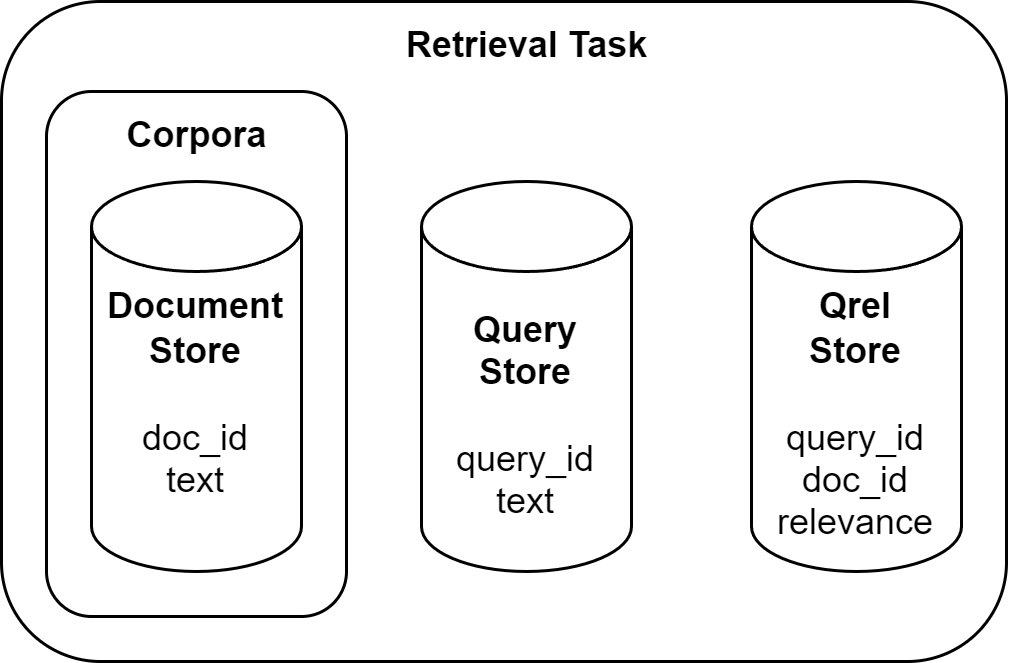
\includegraphics[width=0.7\textwidth]{./graphics/drawio/datasets.png}
    \caption{image}
  \end{figure}

\begin{table}[h!]
    \centering
    \footnotesize
    \caption{List of source datasets and their associated retrieval tasks from which existing \texttt{qrels} where transferd into the target dataset \texttt{ClueWeb22/b}.}
    \label{tab:datasets}
    \begin{tabular}{crcrrr}
        \toprule
        \multicolumn{2}{c}{\textbf{Corpus}} & \multicolumn{4}{c}{\textbf{ Associated Retrieval Tasks}} \\
        \cmidrule(lr){1-2} \cmidrule(lr){3-6}
        Name & documents  & Name & Queries &\texttt{qrels} & Labels \\
        \toprule
        
        Args.me & 0.4~m & Touché 2020 Task 1 & 49 & 2,298 & 3 \\
        \midrule

        \multirow{4}{*}{ClueWeb09} & \multirow{4}{*}{1.0~b} & TREC 2009 Web Track & 50 & 23,601 & 3 \\
        & & TREC 2010 Web Track & 50 & 25,329 & 4 \\
        & & TREC 2011 Web Track & 50 & 19,381 & 4\\
        & & TREC 2012 Web Track & 50 & 16,055 & 5 \\
        \midrule

        \multirow{4}{*}{ClueWeb12} & \multirow{4}{*}{731.7~m} & TREC 2013 Web Track & 50 & 14,474 & 5 \\
        & & TREC 2014 Web Track & 50 & 14,432 & 5 \\
        & & Touché 2021 Task 2 & 50 & 2,076 & 3 \\
        & & Touché 2022 Task 2 & 50 & 2,107 & 3 \\
        \midrule

        \multirow{3}{*}{Disks4+5} & \multirow{3}{*}{0.5~m} & Robust04 & 250 & 311,410 & 3 \\
        & & TREC-7 & 50 & 80,345 & 2 \\
        & & TREC-8 & 50 & 86,830 & 2 \\
        \midrule

        \multirow{2}{*}{MS MARCO} & \multirow{2}{*}{3.2~m} & TREC 2019 DL Track & 43 & 16,258 & 4 \\
        & & TREC 2020 DL Track & 45 & 9,098 & 4 \\
        
        \bottomrule
    \end{tabular}
\end{table}

To simplify data handling, I used \texttt{ir\_datasets}~\citep{macavaney:2021}, a Python package that provides numerous datasets and their associated retrieval tasks. The advantage of \texttt{ir\_datasets} is that it provides a standardized interface for accessing data. Using various iterators, the package manages access to corpora, queries, and \texttt{qrels}, enabling the transfer pipeline to handle different datasets in a uniform way. The datasets and retrieval tasks used in this research are listed in Table~\ref{tab:datasets}. The source datasets were selected because they are widely used in the field of information retrieval and because each dataset comes up with associated retrieval tasks in \texttt{ir\_datasets}. The retrieval tasks, providing \texttt{qrels} for the source datasets, are later transferd to the target dataset, \texttt{ClueWeb22/b}. The target dataset, \texttt{ClueWeb22/b}, was chosen because it is currently the newest ClueWeb corpus in the \texttt{Lemur Project}\footnote{https://lemurproject.org}. The corpus is significantly large, containing over 1.0~billion documents. Due to its size, the ratio of \texttt{qrels} to documents is relatively low. Therefore, the goal is to transfer the existing \texttt{qrels} from the source datasets and their associated retrieval tasks to generate new \texttt{qrels} for \texttt{ClueWeb22/b}, thereby enriching the corpus with additional relevance judgments. 


% =====================
% Document Segmentation
% =====================
\section{Document Segmentation}\label{document-segmentation}

After selecting the datasets and their associated retrieval tasks, including the queries and \texttt{qrels}, the first step in the transfer pipeline is the segmentation of documents from the source datasets into passages. This step was done because the relevance of a document is often confined to specific sections rather than the entire text. By segmenting documents into passages, the pipeline can focus solely on the relevant passages, disregarding non-relevant parts of a document in the subsequent processing.

% Document Selection
\subsection{Document Selection}\label{document-selection}

Instead of segmenting the entire source dataset, only a selection of documents is needed. The workflow begins by selecting only already judged documents from the source dataset. A document is considered judged if it contains at least one relevance assessment in the \texttt{qrels} of the associated retrieval task. Only these documents are suitable for relevance transfer, as their relevance has already been determined. Documents without relevance judgments are excluded, as they provide no usable information for the transfer procedure.
\\\\
As shown in Table~\ref{tab:datasets}, the number of possible relevance label values varies across retrieval tasks. Some tasks use binary labels, such as \textit{"not relevant"} (label 0) and \textit{“relevant”} (label 1). Others employ a Likert scale, distinguishing between levels such as \textit{“relevant”} and \textit{“highly relevant”}. Tasks with additional gradations for non relevant \texttt{qrels}, such as \textit{"not relevant"} (label 0) and \textit{"negatively relevant”} (label -1), were standardized during processing. Labels smaller than 0 were mapped to \textit{"not relevant"} (label 0). \textcolor{red}{This standardization was applied because the metrics used in this study, e.g., \texttt{precision@10}, do not differentiate between different levels of not relevant}.
\\\\
So far, all documents with at least one relevance assessment for any query of the retrieval task are identified. For each query and each possible label value in the retrieval task, all documents matching the query-label combination are determined. These documents are then assigned to the corresponding query-label pairs. Large retrieval tasks, such as Robust04 with over 300,000~\texttt{qrels}, contain many documents for each query-label pair. Therefore, the number of documents per query-label pair is limited. The pairs are used to identify for each query the label with the fewest docuemtns. The number of documents for each query-label pair is then set to the determined minimum, up to a maximum of 50 documents. 
\\\\
This limit reduces processing effort while ensuring that only a representative subset of judged documents is used for relevance transfer. The reason for limiting the number of documents per label for each query to the minimum frequency per query-label combination is to standardize the number of representative documents per label for each query. This avoids that the relevance transfer is biased towards a specific label in the transfer process.

% Segmentation with spaCy
\subsection{Segmentation with spaCy}\label{segmentation-with-spacy}

Once the documents are selected, they are segmented into passages to facilitate further processing. For this purpose, the GitHub repository grill-lab/trec-cast-tools\footnote{https://github.com/grill-lab/trec-cast-tools} was utilized. This repository provides a suite of scripts specifically designed for processing TREC CAst tracks. Among its features is a wrapper class for document segmentation that leverages the capabilities of the \texttt{spaCy}\footnote{https://spacy.io} library, a powerful tool for Natural Language Processing (NLP) in Python.
\\\\
The segmentation workflow employs \texttt{spaCy's} SentenceRecognizer\footnote{https://spacy.io/api/sentencerecognizer} component, which divides text into sentences. First, the wrapper class uses the SentenceRecognizer pipeline to split the documents into sentences. Then, the returned sentences from \texttt{spaCy} are concatenated into passages, each limited to a maximum size of 250 words. As a result, each document is transformed into a series of uniquely identifiable passages. These identifiers consist of the original document ID combined with an additional passage ID, ensuring traceability throughout the transfer pipeline.
\\\\
The documents from the source dataset, selected in the first step, are now available as uniquely passages. In the next stage of the transfer pipeline, these individual passages are classified. In cases where a document is judged as relevant to a query, the relevant information is often dispersed throughout the text. To address this, the transfer pipeline identifies the passages with a high density of relevant information. This step is essential for optimizing the results of the pairwise preferences in the final stage. It ensures that the most relevant and non-relevant passages are accurately identified for each query.


% ===============
% Passage Scoring
% ===============
\section{Passage Scoring}\label{passage-scoring}

In the first step of the transfer pipeline, a subset of the documents from the corpus was segmented into passages. Only documents with at least one relevance assessment in the \texttt{qrels} of the retrieval task were considered for selection. This was done to transfer the information from existing relevance assessments in subsequent stages of the pipeline. To determine which passages of a document best reflect the relevance label from a \texttt{qrel}, i.e., \texttt{(query, document, relevance)} triple, and which passages are most relevant to a query, a ranking of the individual passages is performed in this step.
\\\\
As detailed in Section~[\nameref{selection-documents}], each query-label combination of the retrieval task has an associated set of \texttt{qrels}. To evaluate all passages of the selected documents associated to a query-label combination, the following procedure is applied. First, each passage of a selected document is treated independently and submitted as a query to the source dataset. Then, based on the retrieved ranking of documents for this query, the relevance of the passage is computed using \texttt{precision@10} and \texttt{nDCG@10}.
\\\\
\textbf{Precision} is the fraction of retrieved documents that are relevant to the requested information. In this context, the requested information is the query of the \texttt{qrel} of the retrieval task to which the document is assigned, regardless of whether the document is labeled relevant or non-relevant to the query. Restricting the evaluation to \texttt{precision@10} ensures that only the top 10 retrieved documents are considered. The result of this evaluation is assigned as a score to the query-passage combination.
\\\\
\textbf{Normalized Discounted Cumulative Gain} (\texttt{nDCG}) is another metric commonly used in information retrieval to evaluate the quality of a ranking. Cumulative Gain (\texttt{CG}) represents the sum of all relevance labels for the retrieved document ranking. Again, the query of the retrieval task to which the document is assigned serves for determining the labels of the retrieved documents. Unlike \texttt{precision}, \texttt{CG} considers the label values instead of simply differentiating between non-relevant and relevant labels. This provides greater granularity in retrieval tasks with more than two labels, enabling more nuanced scoring of the passages of a document. The advanced Discounted Cumulative Gain (\texttt{DCG}) further refines this evaluation. It introduces a positional factor to the ranking. It assigns higher weight to relevant results that appear earlier in the ranking. The final score, \texttt{nDCG}, is calculated by normalizing the \texttt{DCG} score with the \texttt{Ideal DCG} (\texttt{IDCG}), which represents the optimal theoretical ranking for the query. As for \texttt{precision}, the evaluation is limited to the first 10 documents by calculating \texttt{nDCG@10}.
\\\\
Passages with a high density of information relevant to a inforamtion need are theoretically more likely to retrieve relevant documents and  for that achieve higher scores on the metrics described above. Conversely, passages that contribute minimal or no relevant information to a inforamtion need result in lower scores due to fewer retrieved relevant documents.
\\\\
Since this study does not aim to optimize or analyze a specific set of retriever systems but uses them for passage scoring, a diverse selection of models was employed to minimize bias in the scores that could arise from relying on a single model. For that reason \texttt{Precision} and \texttt{nDCG} scores were calculated using the following retriever systems: \texttt{BM25, DFR\_BM25, DFIZ, DLH, DPH, DirichletLM, Hiemstra\_LM, LGD, PL2, and TF\_IDF}. An evaluation of which model best scores the passages in relation to the goal of relevance transfer follows in Chapter~\ref{evaluation}~[\nameref{rank-correlation-passage-scores}].
\\\\
In this pipeline stage, the individual passages of the selected documents belonging to the query-label pairs were scored. These scores will be the basis for the subsequent steps to identify candidates from the target dataset. The selected candidates will get new relevance assessments inferred at the end of the pipeline. Furthermore, these scores will determine the known passages from the source dataset, used in pairwise preferences alongside the candidates.


% ====================
% Candidate Retreiaval
% ====================
\section{Candidate Selection}\label{candidate-selection}

This section outlines the methods used to select candidates for the pairwise preference inference. A candidate consists of a passage from the source dataset, a passage from the target dataset, and a query from a retrieval task, i.e. \texttt{(source passage, target passage, query)}. The goal is to score each candidate using pairwise preferences to infer new relevance assessments for a set of target documents. The process begins with selecting document with retrieval from the target dataset.

% Document Retrieval from Target Dataset
\subsection{Document Retrieval from Target Dataset}\label{document-retrieval-from-target-dataset}

For each query in a retrieval task of a source dataset, a set of documents from the target dataset is retrieved. The aim is to identify documents most likely to be relevant to the query. For that, all strategies employ \texttt{BM25} model for retrieval due to its simplicity and efficiency \textcolor{red}{REF\_PAPER}. Since this step only requires a preliminary selection of potentially relevant documents, \texttt{BM25} is sufficient for this task. A fine-grained relevance classification is performed later through the pairwise preferences. Chapter~\ref{evaluation}~[\nameref{candidate-selection}] evaluates these strategies to assess their effectiveness in identifying relevant documents.
\\\\
\textbf{Naive Approach}
The first approach, termed \texttt{naive}, involves submitting each query from the retrieval task to the target dataset corpus to generate a ranking of potentially relevant documents. From this ranking, the top 1000 documents are initially assigned as candidates. Unfortunately, some search queries include ambiguities, leaving room for interpretation regarding the intended information. For example, the query \textit{``Apple``} could refer to either the technology brand or the fruit. To address such ambiguities, the query description of each query is included in the retrieval process. A query description is a brief text that provides additional context, clarifying the search intent and specifying the query's focus. The query description is treated as an independent query and also submitted to the corpus, retrieving an additional top 1000 documents based on the BM25 ranking. After filtering out duplicates between the two sets, up to 2000 unique documents per query are selected for further processing.
\\\\
\textbf{Nearest Neighbor Approach}
The second approach, \texttt{nearest neighbor}, builds on the relevant documents identified in the initial pipeline step descripted in Chapter~\ref{methodology}~[\nameref{document-selection}]. The passages of all selected documents of a query are now used as independent queries to retrieve documents from the target dataset. From the resulting rankings, the top 20 documents are added to the candidate set for the corresponding query. This process is repeated for all passages of all relevant documents. As a result, each passage can contribute up to 20 unique documents to the candidate set.
\\\\
\textbf{Union Approach}
The third approach, called \texttt{union}, combines the \texttt{naive} and \texttt{nearest neighbor} approaches into a single candidate set for each query. This combination is intended to enhance the \texttt{Recall} of the number of retrieved relevant docuements by including a broader set of potentially relevant documents. However, the increased number of documents may reduce \texttt{Precision} by including more irrelevant entries, thereby increasing the workload for pairwise preference evaluations in later stages. The \texttt{Recall} and \texttt{Precision} of the approaches are evaluated in Chapter~\ref{evaluation}~[\nameref{candidate-selection}].

% Postprocessing of Selected Target Documents
\subsection{Postprocessing of Selected Target Documents}\label{postprocessing-of-selected-target-documents}
As described in Section~\nameref{segmentation-with-spacy}, selected documents from the source dataset are segmented into passages for later processing. Since pairwise preferences will be applied at passage level, documents from both the source and target datasets have to be divided into passages. This is done using the same process as outlined before. First, \texttt{spaCy} is employed for segmenting the chosen target documents into sentences, and then passages are formed by concatenating sentences.

% Composing Final Candidates
\subsection{Composing Final Candidates}\label{composing-final-candidates}
As mentioned before, a candidate comprises a passage from the source dataset, a passage from the target dataset, and a query provided by a retrieval task. The queries are provided by the retrieval task which is used to facilitate the transfer of its existing \texttt{qrels}. The documents from the target dataset, along with their associated passages, are identified as just described. To conduct pairwise preference comparisons, passages from the source dataset need to be selected. The objective is to compare each selected passage from the target dataset for a given query against 15 relevant and 5 non-relevant passages from the source dataset corresponding to the same query. To determine the relevant and non-relevant passages, the computed scores of the previous pipeline stage, Section~\nameref{passage-scoring}, are used. The selection is made using two different strategies referred to as \texttt{simple selection} and \texttt{diversified selection}.
\\\\
\textbf{Simple Selection}
During the \nameref{passage-scoring} stage, each selected passage from the source dataset is evaluated and assigned scores based on the \texttt{precision@10} and \texttt{nDCG@10} metrics. These scores are now used to generate a ranking for each query. Following this strategy, the 15 highest-scoring passages and the 5 lowest-scoring passages for each query are selected.
\\\\
\textbf{Diversified Selection}
It is possible that the top- and lowest-rated passages are predominantly drawn from a small subset of documents. While such passages may satisfy the selection criteria of the \texttt{simple selection}, this concentration could lead to unintended side effects by limiting variation in the pairwise preferences. To mitigate potential bias because of reduced document diversity, this approach restricts the selection to a maximum of one passage per document. Specifically, it selects the top 15 and bottom 5 passages for each query, ensuring that each passage is sourced from a distinct document. This strategy enhances diversity in pairwise preference comparisons by incorporating a wider range of source documents.
\\\\
For each query, 20 selected passages from either the \texttt{simple} or \texttt{diversified selection} approach are carried forward to the final pipeline stage. These candidates will go through pairwise preference evaluations to infer new relevance assessments for the selected target dataset documents.

% ====================
% Pairwise Preferences
% ====================
\section{Pairwise Preferences}\label{pairwise-transfering-relevance-labels-across-datasets}

At this stage, all necessary processing steps have been completed to perform the pairwise preferences. The transfer pipeline began with selecting a subset of documents from the source corpus for each query. These documents were segmented into passages, and each passage was scored by treating it as an independent query against the source corpus. The retrieved document rankings were used to compute \texttt{precision} and \texttt{nDCG} metrics, which were then assigned as passage scores. The highest-scoring passages guided the selection of candidates for the pairwise preferences, which is now described in detail.
\\\\
A candidate is defined as a combination of three elements: a query from a retrieval task of the source dataset, a known passage from a source dataset document, and a passage to judge from a target dataset document. The query is predefined by the retrieval task, while the known passage was identified during the initial document selection step. The passage to judge was determined in the candidate retrieval step. The known passage serves as a reference for comparison and can either be relevant or non-relevant. The objective of the pairwise preference evaluation is to assess the relevance of the passage to judge with respect to the query by comparing it to the known passage.
\\\\
The \texttt{autoqrels}\footnote{https://github.com/seanmacavaney/autoqrels} GitHub repository was used to perform pairwise preference. \texttt{autoqrels} is a tool designed to automatically infer query relevance assessments (qrels), supporting zero-shot and one-shot labeling. The original \texttt{autoqrels} paper~\citep{macavaney:2023} evaluated the capability of one-shot labelers for automatic relevance estimation. Among the evaluated approaches, the \texttt{DuoPrompt} method which uses the \texttt{FLAN-T5} model demonstrated superior performance compared to the other tested systems \texttt{DuoT5}, {MaxRep-TCT} and \texttt{MaxRep-TCT}. Therefore, for this thesis, the one-shot labeling with \texttt{DuoPrompt} was utilized to perform the pairwise preference inference.
\\\\
\texttt{FLAN-T5} is a Text-to-Text Transfer Transformer model that is an advanced version~\citep{chung:2022} of Google's \texttt{T5} model. While the backbone architecture of \texttt{FLAN-T5} remains \texttt{T5}, it has been further fine-tuned on an expansive and diverse set of training tasks, enhancing its performance across a wide range of natural language processing tasks. \texttt{FLAN-T5} is available in various sizes, ranging from smaller, resource-efficient versions like \texttt{flan-t5-small}, with 80~million parameters, to much larger models such as \texttt{flan-t5-xxl} with 11~billion parameters, accommodating different computational and application needs. For this thesis, given the constraints in computational resources, the \texttt{flan-t5-base}\footnote{https://huggingface.co/google/flan-t5-base} model with 250 million parameters is used as the DuoPrompt model.
\\\\
\begin{figure}[ht]
    \centering
    \begin{tcolorbox}[title=One-Shot Prompt]
        \footnotesize
        \begin{verbatim}
PROMPT = (
    "Determine if passage B is as relevant as passage A "
    "for the given query. "
    'Passage A: "...{{ rel_doc_text | replace("\\"", "\'") }}..." '
    'Passage B: "...{{ unk_doc_text | replace("\\"", "\'") }}..." '
    'Query: "{{ query_text }}" '
    "Is passage B as relevant as passage A? </s>"
)
        \end{verbatim}
    \end{tcolorbox}
    \caption{One-shot prompt used for the \texttt{FLAN-T5} model.}
    \label{fig:oneshot-prompt}
\end{figure}

In Figure~\ref{fig:oneshot-prompt} is the prompt structure which is given to \texttt{FLAN-T5}. The prompt takes the query, the known passage (referred to as rel\_doc\_text), and the passage to judge (referred to as unk\_doc\_text) as inputs for pairwise inference. The model then predicts the likelihood that the passage to judge is as relevant to the query as the known passage. If the passage to judge is highly relevant to the query, the model outputs a score close to 1.0. Conversely, if the passage to judge is not relevant, the model produces a score close to 0.0. This process enables a detailed comparison of passage relevance, forming the foundation for inferring new relevance assessments for documents in the target dataset.
\\\\
All candidates are processed through pairwise preference inference, where each passage to judge is compared against 20 known passages as outlined in Section~\ref{composing-final-candidates}. The pairwise preference inferences generate 20 relevance scores for each passage to judge, with higher scores indicating greater relevance to the query associated with the candidate.
\\\\
This chapter provided a detailed description of all steps in the transfer pipeline, resulting in a set of relevance scores for each passage to judge. These scores represent the transferred information from the source dataset, specifically the qrels of a retrieval task, to the target dataset. The next chapter will evaluate the effectiveness of the transfer pipeline and its individual steps.